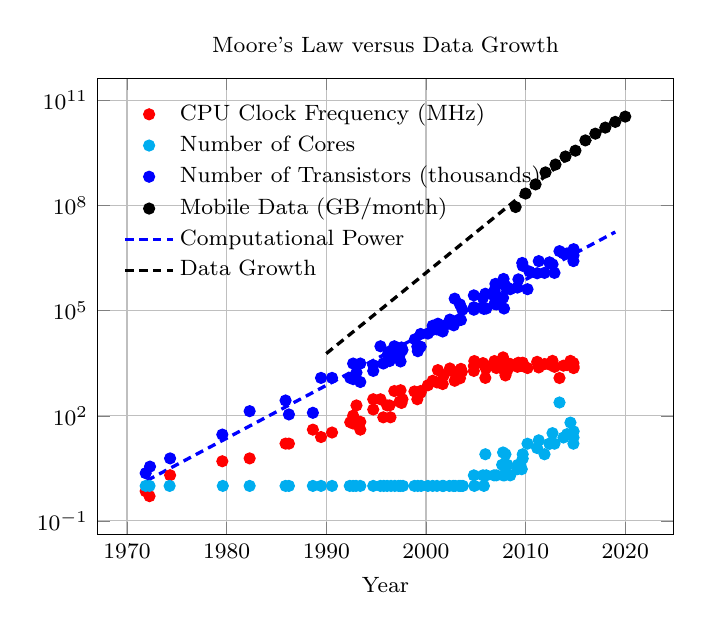
\begin{tikzpicture}
\pgfkeys{/pgf/number format/set thousands separator = {}}
\begin{semilogyaxis}[%
font=\footnotesize,
width=3.5in,
height=2.9in,
xmajorgrids,
ymajorgrids,
title={Moore's Law versus Data Growth},
xlabel={Year},
legend entries={CPU Clock Frequency (MHz), Number of Cores, Number of Transistors (thousands), Mobile Data (GB/month), Computational Power, Data Growth},
legend style={fill=none},
legend style={draw=none},
legend cell align=left,
legend pos=north west
]

%Time, Frequency
\addplot [color=red, mark=*, only marks]
coordinates {
(1971.875,0.704135515) (1972.259615,0.509367522) (1974.326923,2.016914555) (1979.567308,5.048065717) (1982.307692,6.097562352) (1985.913462,16.10761535) (1986.25,16.10761535) (1988.653846,40.31519363) (1989.471154,24.80454414) (1990.576923,33.37624694) (1992.403846,65.52488237) (1992.692308,60.42963902) (1992.692308,100.9035045) (1993.028846,198.0956779) (1993.413462,67.31703824) (1993.413462,40.31519363) (1994.711538,151.2472545) (1994.711538,296.9314848) (1995.432692,296.9314848) (1995.721154,90.57977759) (1996.105769,198.0956779) (1996.346154,198.0956779) (1996.442308,90.57977759) (1996.826923,509.3675217) (1997.355769,252.5478933) (1997.451923,537.6117475) (1997.548077,232.9096592) (1997.644231,296.9314848) (1998.846154,495.8068242) (1999.134615,296.9314848) (1999.182692,399.5420559) (1999.471154,457.2526699) (1999.471154,509.3675217) (2000.192308,743.1795488) (2000.673077,1000) (2001.105769,897.6871324) (2001.201923,2016.914555) (2001.682692,805.8421878) (2001.778846,1420.18117) (2002.403846,2246.790092) (2002.788462,1810.558243) (2002.884615,1000) (2003.413462,1175.743266) (2003.509615,2186.974655) (2003.605769,1810.558243) (2004.807692,2641.64832) (2004.807692,1910.952975) (2004.855769,3651.741273) (2005.721154,3190.848981) (2005.865385,2788.126665) (2005.961538,1207.900747) (2006.009615,2246.790092) (2006.875,3651.741273) (2006.875,2641.64832) (2007.019231,2713.899431) (2007.067308,2308.241527) (2007.644231,2942.727176) (2007.740385,4655.525931) (2007.740385,4067.944321) (2007.836538,2016.914555) (2007.980769,1420.18117) (2008.173077,2016.914555) (2008.173077,2308.241527) (2008.461538,3023.213025) (2009.182692,2502.865431) (2009.278846,3278.121151) (2009.423077,2641.64832) (2009.663462,2641.64832) (2009.711538,3278.121151) (2010.192308,2308.241527) (2011.16,3470) (2011.32,2400) (2011.9,3000) (2012.4,3100) (2012.41,2900) (2012.7,3700) (2012.9,2500) (2013.4,1200) (2013.8,2700) (2014.16,2800) (2014.5,3700) (2014.8,3200) (2014.81,2600) (2014.82,2300) };

%Time, Cores
\addplot [color=cyan, mark=*, only marks]
coordinates {
(1971.875,1) (1972.259615,1) (1974.278846,1) (1979.615385,1) (1982.307692,1) (1985.913462,1) (1986.25,1) (1988.653846,1) (1989.471154,1) (1990.576923,1) (1992.355769,1) (1992.692308,1) (1992.980769,1) (1993.413462,1) (1994.711538,1) (1995.432692,1) (1995.769231,1) (1996.105769,1) (1996.490385,1) (1996.875,1) (1997.259615,1) (1997.451923,1) (1997.692308,1) (1998.846154,1) (1999.182692,1) (1999.519231,1) (2000.192308,1) (2000.673077,1) (2001.105769,1) (2001.634615,1) (2001.778846,1) (2002.355769,1) (2002.740385,1) (2002.932692,1) (2003.317308,1) (2003.509615,1) (2003.701923,1) (2004.807692,2) (2004.855769,1) (2005.721154,2) (2005.817308,1) (2005.961538,8) (2006.057692,2) (2006.826923,2) (2007.067308,2) (2007.644231,4) (2007.740385,9) (2007.740385,2) (2007.884615,2) (2007.980769,8) (2008.173077,4) (2008.461538,2) (2009.182692,3) (2009.230769,4) (2009.471154,4) (2009.615385,3) (2009.711538,8) (2009.711538,6) (2010.192308,16) (2011.16,12) (2011.32,20) (2011.9,8) (2012.4,16) (2012.41,16) (2012.7,32) (2012.9,16) (2013.4,240) (2013.8,24) (2014.16,30) (2014.5,64) (2014.8,16) (2014.81,24) (2014.82,36) };


%Time, Transistors
\addplot [color=blue, mark=*, only marks]
coordinates {
(1971.875,2.308241527) (1972.307692,3.554522356) (1974.326923,6.097562352) (1979.567308,29.16377574) (1982.307692,135.7727142) (1985.913462,273.8419634) (1986.25,109.4113811) (1988.653846,121.8814185) (1989.471154,1207.900747) (1990.576923,1207.900747) (1992.403846,1207.900747) (1992.692308,3105.900224) (1992.692308,1113.97386) (1993.028846,1715.437896) (1993.413462,3105.900224) (1993.413462,922.2395651) (1994.711538,1910.952975) (1994.711538,2788.126665) (1995.432692,9646.616199) (1995.721154,3105.900224) (1996.153846,5473.703263) (1996.346154,6792.52507) (1996.346154,3651.741273) (1996.442308,4293.51021) (1996.826923,9646.616199) (1997.355769,5473.703263) (1997.451923,3554.522356) (1997.548077,8896.491128) (1997.644231,7566.695371) (1998.894231,15261.37803) (1999.134615,9389.79801) (1999.182692,6978.305849) (1999.471154,9389.79801) (1999.471154,21673.9217) (2000.192308,22266.7201) (2000.673077,28387.35965) (2000.673077,37180.26664) (2001.105769,29163.77574) (2001.201923,42550.65502) (2001.682692,25482.96748) (2001.826923,37180.26664) (2002.403846,55730.60401) (2002.788462,38197.17549) (2002.884615,220673.4069) (2003.413462,151247.2545) (2003.509615,54246.90937) (2003.653846,106498.5635) (2004.807692,125214.9689) (2004.807692,106498.5635) (2004.807692,273841.9634) (2005.721154,232909.6592) (2005.817308,112403.8664) (2005.961538,305052.789) (2006.057692,115478.1985) (2006.875,378551.5249) (2006.875,155383.9831) (2006.923077,245824.4069) (2006.971154,296931.4848) (2006.971154,582941.5347) (2007.067308,151247.2545) (2007.644231,582941.5347) (2007.740385,232909.6592) (2007.788462,805842.1878) (2007.836538,115478.1985) (2007.980769,509367.5217) (2008.221154,445079.4062) (2008.461538,410469.838) (2009.182692,457252.6699) (2009.278846,784388.5581) (2009.663462,2308241.527) (2009.711538,1910952.975) (2010.192308,410469.838) (2010.384615,1309747.264) (2011.16,1170000) (2011.32,2600000) (2011.9,1200000) (2012.4,2400000) (2012.41,2300000) (2012.7,2100000) (2012.9,1200000) (2013.4,5000000) (2013.8,4300000) (2014.16,4300000) (2014.5,4200000) (2014.8,2600000) (2014.81,3800000) (2014.82,5700000) };

\addplot [color=black, mark=*, only marks]
coordinates {
(2009, 91000000) (2010, 220000000) (2011, 402000000) (2012, 884000000) (2013, 1480000000) (2014, 2514000000) (2015, 3685000000) (2016, 7241000000) (2017, 11266000000) (2018, 16792000000) (2019, 24452000000) (2020, 34588000000) };

\addplot [color=blue, densely dashed, line width=1.2pt]
coordinates {
(1972, 1.42192406e+00) (1973, 2.01272654e+00) (1974, 2.84900455e+00) (1975, 4.03275198e+00) (1976, 5.70834066e+00) (1977, 8.08012823e+00) (1978, 1.14373819e+01) (1979, 1.61895580e+01) (1980, 2.29162401e+01) (1981, 3.24378255e+01) (1982, 4.59155830e+01) (1983, 6.49932828e+01) (1984, 9.19976733e+01) (1985, 1.30222256e+02) (1986, 1.84328965e+02) (1987, 2.60916746e+02) (1988, 3.69326375e+02) (1989, 5.22779674e+02) (1990, 7.39992067e+02) (1991, 1.04745514e+03) (1992, 1.48266762e+03) (1993, 2.09870875e+03) (1994, 2.97071196e+03) (1995, 4.20502822e+03) (1996, 5.95219683e+03) (1997, 8.42530545e+03) (1998, 1.19259786e+04) (1999, 1.68811642e+04) (2000, 2.38952052e+04) (2001, 3.38235459e+04) (2002, 4.78770634e+04) (2003, 6.77697486e+04) (2004, 9.59277471e+04) (2005, 1.35785256e+05) (2006, 1.92203364e+05) (2007, 2.72062920e+05) (2008, 3.85103730e+05) (2009, 5.45112443e+05) (2010, 7.71603991e+05) (2011, 1.09220167e+06) (2012, 1.54600611e+06) (2013, 2.18836407e+06) (2014, 3.09761862e+06) (2015, 4.38466397e+06) (2016, 6.20647036e+06) (2017, 8.78522838e+06) (2018, 1.24354477e+07) (2019, 1.76023153e+07)};

\addplot [color=black, densely dashed, line width=1.2pt]
coordinates {
(1990, 5.96878326e+03) (1991, 1.01461770e+04) (1992, 1.72472182e+04) (1993, 2.93180907e+04) (1994, 4.98370478e+04) (1995, 8.47166811e+04) (1996, 1.44007648e+05) (1997, 2.44794797e+05) (1998, 4.16120209e+05) (1999, 7.07351751e+05) (2000, 1.20240856e+06) (2001, 2.04394254e+06) (2002, 3.47444393e+06) (2003, 5.90611546e+06) (2004, 1.00396496e+07) (2005, 1.70661352e+07) (2006, 2.90102724e+07) (2007, 4.93137958e+07) (2008, 8.38272187e+07) (2009, 1.42495675e+08) (2010, 2.42224633e+08) (2011, 4.11751255e+08) (2012, 6.99925082e+08) (2013, 1.18978416e+09) (2014, 2.02248266e+09) (2015, 3.43796485e+09) (2016, 5.84410562e+09) (2017, 9.93424077e+09) (2018, 1.68869535e+10) (2019, 2.87056861e+10) };

\end{semilogyaxis}
\end{tikzpicture}